\section{Results}
\label{sec:results}

Each figure and table is regenerated from the \texttt{metrics.csv} of its experiment (scripts in
\texttt{papers/shared/figures}).

\subsection{The decimation valley on Ottawa and its captor}
\label{sec:res-valley}

Table~\ref{tab:ottawa} and Fig.~\ref{fig:valley} give the order hits of the outer race under pure
decimation, with the 25~kHz search ceiling.
\begin{itemize}
  \item At full rate the classical pipeline hits 27 of 36 segments under the nested ruler and 31 of
  35 under the local ruler.
  \item Decimation by 3 to 6 brings both down to 2--11 hits. The valley closes again at $8\times$,
  with 25 and 28 hits.
  \item The inner race is not affected: it stays at 35--36 of 36 hits in every cell, under both
  rulers.
\end{itemize}

The selected band shows where the loss comes from. At full rate the kurtogram selects a band
between 2.0 and 4.6~kHz in 32 of the 36 outer-race segments, and a band above 12.75~kHz in 2. At
$4\times$ the raw records move it to $[12.75, 25]$~kHz, the band that receives the three folding
zones of Section~\ref{sec:zones}, in 26 of 36 segments, and above 12.75~kHz in 29.

Removing the single-sample spikes before decimation closes the valley, and the selection at
$4\times$ returns to the band chosen at full rate (3 of 36 above 12.75~kHz).
\begin{itemize}
  \item At $4\times$ the pipeline hits 28 of 36 segments against 6, with all 22 discordant pairs in
  favour (exact McNemar, $p = 4.8\times10^{-7}$). Under the local ruler it hits 32 of 35
  ($p = 3\times10^{-8}$).
  \item Because the three segments of a record are not independent, the comparison was repeated
  at record level as a sensitivity analysis: 11 of the 12 outer-race records improve and none
  worsens (exact sign test, $p = 0.001$).
  \item The three-point median gives the same counts up to $4\times$, and the ideal anti-alias filter
  gives 27 hits at every factor up to $5\times$.
\end{itemize}

The zone rejections attribute the loss at $4\times$. Rejecting $Z_1$ alone leaves 7 hits against
6, rejecting $Z_2$ or $Z_3$ alone recovers 21, and rejecting the three recovers 27, the same as the
ideal anti-alias filter. Lowering the search ceiling to 12.5~kHz also avoids the valley: the
raw records then stay at 27--29 hits from $1\times$ to $6\times$.

\begin{table}[t]
  \centering
  \caption{Outer-race order hits on Ottawa under pure decimation, with the 25~kHz search ceiling
  unless stated. Each cell gives the hits under the nested ruler (of 36 segments) and, in
  parentheses, under the local ruler (of 35; one segment has no valid full-rate line). The zones
  are the original-frequency intervals that fold onto $[12.75, 25]$~kHz at $4\times$.}
  \label{tab:ottawa}
  \small
  % gerado por papers/shared/figures/tab_ottawa_valley.py a partir de
% experiments/E20-fold-zone-rejection/results/metrics.csv; nao editar a mao.
% celula: acertos na regua aninhada (de 36) e, entre parenteses, na local (de 35)
\begin{tabular}{lccccccc}
\toprule
 & \multicolumn{7}{c}{decimation factor $M$} \\
\cmidrule(lr){2-8}
intervention before decimation & 1$\times$ & 2$\times$ & 3$\times$ & 4$\times$ & 5$\times$ & 6$\times$ & 8$\times$ \\
\midrule
raw, no intervention & 27 (31) & 20 (22) & 4 (4) & 6 (6) & 2 (2) & 11 (11) & 25 (28) \\
reject $Z_1$ (25--37.25~kHz) & 27 (31) & 20 (22) & 4 (4) & 7 (7) & 3 (3) & 12 (12) & 25 (28) \\
reject $Z_2$ (62.75--75~kHz) & 27 (31) & 20 (22) & 4 (4) & 21 (24) & 12 (13) & 12 (12) & 26 (29) \\
reject $Z_3$ (75--87.25~kHz) & 27 (31) & 28 (32) & 19 (21) & 21 (24) & 2 (2) & 24 (27) & 26 (29) \\
reject $Z_1 \cup Z_2 \cup Z_3$ & 27 (31) & 28 (32) & 21 (23) & 27 (31) & 15 (16) & 23 (26) & 29 (32) \\
ideal anti-alias filter & 27 (31) & 27 (31) & 27 (31) & 27 (31) & 27 (29) & 25 (28) & 27 (30) \\
single-sample spikes removed & 28 (32) & 28 (32) & 28 (32) & 28 (32) & 27 (30) & 24 (27) & 29 (32) \\
3-point median & 28 (32) & 28 (32) & 28 (32) & 28 (32) & 25 (28) & 25 (28) & 28 (31) \\
\midrule
raw, search ceiling 12.5~kHz & 27 (30) & 28 (31) & 28 (31) & 29 (32) & 29 (32) & 29 (32) & 25 (28) \\
\bottomrule
\end{tabular}

\end{table}

\begin{figure}[t]
  \centering
  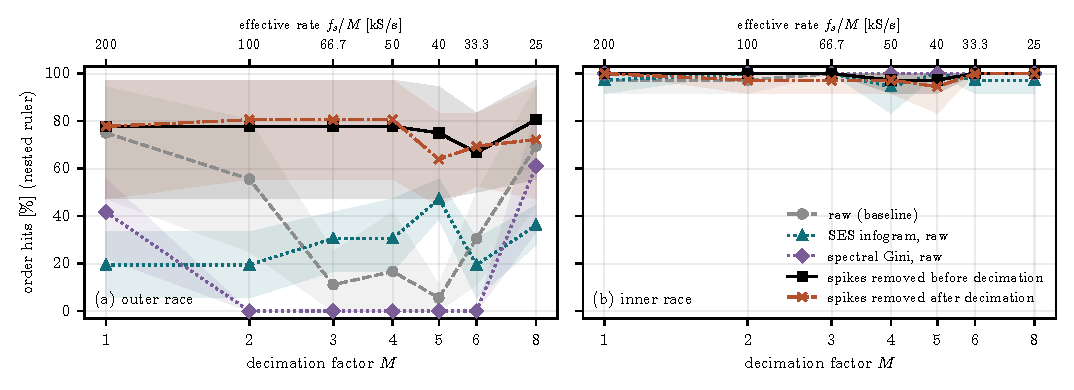
\includegraphics{figures/fig_valley_nested.pdf}
  \caption{Order hits against the decimation factor on Ottawa, under the nested ruler, for the
  outer race (a) and the inner race (b). The shaded bands are 95\% intervals from a bootstrap over
  the four condition-by-scenario clusters of each race; with four clusters they are wide. The top
  axis gives the effective rate.}
  \label{fig:valley}
\end{figure}

\subsection{Injected interference}
\label{sec:res-injected}

CWRU 48k has no native high-band interferer, and its classical baseline degrades monotonically
under decimation. A controlled interferer injected above the 10~kHz search ceiling therefore tests
the mechanism on a second rig (13 drive-end fault records, 12 of the outer race and one of the
inner race). The numbers below come from \texttt{E23/results/paper\_numbers.json}.
\begin{itemize}
  \item Exponentially decaying bursts at 97.7 bursts per second, on carriers between 13 and
  22~kHz, capture the kurtogram under pure decimation at the highest dose. At factors of 2 and
  above, 193 segments are hit without injection and missed with it. In 189 of them (98\%) the
  estimate falls on the burst rate or one of its first three harmonics.
  \item A phase-randomized surrogate of the same realization has the same amplitude spectrum, bin
  by bin, and does not capture. At the lowest dose that captures, its mean loss is 0.14 of that of
  the bursts. The 95\% interval, from a bootstrap over the four independent fault clusters, is
  $[0.03, 0.21]$. For a kurtosis-based selector the capture needs impulsiveness, not only folded
  power.
  \item Trains of single-sample spikes also capture, and the loss grows with their amplitude. Over
  three spike rates, the largest loss at factors of 2 and above is 8--15 points at 8 MAD, 23--31
  at 16 MAD and 46--62 at 32 MAD.
  \item Without injection, the ideal anti-alias filter costs 8.5 points over factors of 2 and above
  (94.0\% to 85.5\%) and 27 points at $10\times$ and $12\times$ (88.5\% to 61.5\%). It removes the
  fault resonance that folding would bring into the search range, the trade-off that motivates
  bandpass sampling \citep{vaughan1991}.
\end{itemize}

Three limits narrow these results.
\begin{itemize}
  \item The highest dose is about 17~dB above the power of the band selected at full rate. The code
  labels it +20~dB because its band-power routine returns half the power.
  \item The 12 outer-race records are one fault size at three positions relative to the load zone
  and four loads, so there are four independent units.
  \item The folded share of the interferer power was pre-registered as the predictor of capture.
  It does not predict the size of the loss among the 48 cells where it predicts capture (Spearman
  $\rho = 0.08$, $p = 0.61$).
\end{itemize}
We therefore report the mechanism and its dependence on impulsiveness, not a predictive rule.

\subsection{Robust selectors against the valley}
\todo[inline]{From E20 with \texttt{config/selectors.yaml}: SES infogram, SES infogram after spike
removal, spectral Gini. Pre-registered recovery criterion at 4$\times$.}

\subsection{Replication on Paderborn}
\todo[inline]{From E24: H1 (spike removal) and H2 (SES infogram) under the nested ruler, with the
local ruler as secondary, and the selected bands.}

\subsection{Can a benchmark detect a learned improvement?}
\todo[inline]{Power gate. Ottawa: power 0.00--0.07 for +5, +10 points and a perfect arm in every
valid design (\texttt{E15/results/power\_gate}); the classical baseline misses only 3--9 of about 60
test segments. Paderborn: power 1.00 at +5 points with three seeds per fold
(\texttt{E15/results-paderborn-gate}).}

\subsection{Learned sampling masks}
\todo[inline]{Ottawa decisive run: no detectable gain in an underpowered design (state it as
absence of evidence; O-C-2 dependence). Paderborn run: pending (\texttt{E15/results-paderborn}).}

\subsection{Where the method fails}
\todo[inline]{Mandatory failure case: bearings whose fault line is invisible at full rate on
Paderborn (17 of 23); the 96--128$\times$ wall of the classical pipeline on Ottawa, where the
selected bands become narrower than the fault frequency.}
